
\documentclass[journal,transmag]{IEEEtran}
\hyphenation{op-tical net-works semi-conduc-tor}

\usepackage{enumitem}

% *** GRAPHICS RELATED PACKAGES ***
%
\ifCLASSINFOpdf
   \usepackage[pdftex]{graphicx}
  % declare the path(s) where your graphic files are
  % \graphicspath{{../pdf/}{../jpeg/}}
  % and their extensions so you won't have to specify these with
  % every instance of \includegraphics
  % \DeclareGraphicsExtensions{.pdf,.jpeg,.png}
\else
  % or other class option (dvipsone, dvipdf, if not using dvips). graphicx
  % will default to the driver specified in the system graphics.cfg if no
  % driver is specified.
  % \usepackage[dvips]{graphicx}
  % declare the path(s) where your graphic files are
  % \graphicspath{{../eps/}}
  % and their extensions so you won't have to specify these with
  % every instance of \includegraphics
  % \DeclareGraphicsExtensions{.eps}
\fi
% graphicx was written by David Carlisle and Sebastian Rahtz. It is
% required if you want graphics, photos, etc. graphicx.sty is already
% installed on most LaTeX systems. The latest version and documentation
% can be obtained at: 
% http://www.ctan.org/pkg/graphicx
% Another good source of documentation is "Using Imported Graphics in
% LaTeX2e" by Keith Reckdahl which can be found at:
% http://www.ctan.org/pkg/epslatex
%
% latex, and pdflatex in dvi mode, support graphics in encapsulated
% postscript (.eps) format. pdflatex in pdf mode supports graphics
% in .pdf, .jpeg, .png and .mps (metapost) formats. Users should ensure
% that all non-photo figures use a vector format (.eps, .pdf, .mps) and
% not a bitmapped formats (.jpeg, .png). The IEEE frowns on bitmapped formats
% which can result in "jaggedy"/blurry rendering of lines and letters as
% well as large increases in file sizes.
%
% You can find documentation about the pdfTeX application at:
% http://www.tug.org/applications/pdftex





\begin{document}

\title{\textsc{Visualizando y entendiendo Bacterias, microalgas y hongos}}

\author{
\IEEEauthorblockN{Daniela Conde Herrera , Danna Sofía Jerez,  Karen Mariana Jiménez, Willia  Andrés Gómez, Fidson Juarismy Vesga}
\IEEEauthorblockA{Pontificia Universidad Javeriana, Bogotá, Colombia}
\IEEEauthorblockA{INFORME 2}
\IEEEauthorblockA{Grupo IV}

}
% The paper headers
\markboth{Microbiología. Octubre 12~2021}%
{Shell \MakeLowercase{\textit{et al.}}: Bare Demo of IEEEtran.cls for IEEE Transactions on Magnetics Journals}
\IEEEtitleabstractindextext{%

	\begin{abstract}
	Durante estas 4 semanas hemos aprendido a realizar diferentes tinciones para visualizar bacterias bajo el microscopio, aprendimos sobre la tinción de Gram y sobre la tinción de Ziehl-Neelsen, entendimos el funcionamiento de la cámara de Neubauer, donde realizamos el conteo de microalgas sobre la zona blanca y roja de la cámara y procedimos a calcular el número estimado de microalgas en 1 mililitro. Además, aprendimos sobre la caracterización morfológica de hongos (micromicetos filamentosos) y levaduras, así como sus formas de cultivo y la forma de diferenciarlas de las bacterias.
	\end{abstract}
	\begin{IEEEkeywords}
	Tinción de Gram, Tinción Ziehl-Neelsen, Cámara de Neubauer, Microalgas, Levaduras.
	 	\end{IEEEkeywords}}



\maketitle
\IEEEdisplaynontitleabstractindextext
\IEEEpeerreviewmaketitle


\section{Objetivos}

\begin{itemize}
	
    \item Reconocer los diferentes colorantes que se utilizan en la coloración de Gram.
    
    \item Adquirir destreza en la realización de la coloración de Gram.  

    \item Diferenciar experimentalmente bacterias Gram positivas de Gram negativas. 
    
    \item Informar correctamente la coloración de Gram.
    
    \item Con base en el fundamento de la tinción de Gram, interpretar los resultados 


	\end{itemize}
%%%%%%%%%%%%%%%%%%%%%%%%%%MARCO TEÓRICO

 
%%%%%%%%%%%%%%%%%%%%%%%%%%METODOLOGIA
\section{Resultados} 

\subsection{\textbf{Tinción de Gram}} 


\paragraph{\large \textit{\textbf{Bacillus subtilis}}}Bacilos Gram positivos 
	\begin{figure}[!h] 
	\center 
	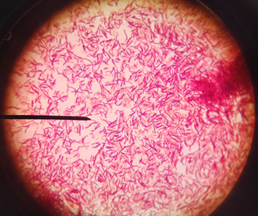
\includegraphics[width=4.2cm]{I1.png} 
	\caption{Imagen de Danna: Tinción de Gram \textit{Bacillus subtilis} } 
	\label{I1}
	\end{figure} 
	\begin{figure}[!h] 
	\center 
	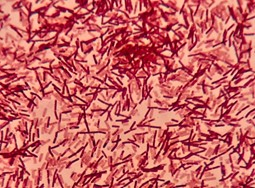
\includegraphics[width=4.2cm]{I5.jpg} 
	\caption{Imagen de Daniela: Tinción de Gram \textit{Bacillus subtilis} } 
	\label{I1}
	\end{figure} 
	\begin{figure}[!h] 
	\center 
	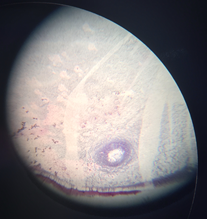
\includegraphics[width=4cm]{I9.png} 
	\caption{Imagen de Karen :Tinción de Gram \textit{Bacillus subtilis} } 
	\label{I1}
	\end{figure} 
	\begin{figure}[!h] 
	\center 
	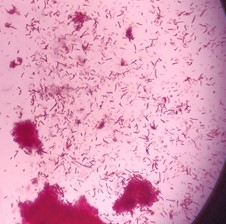
\includegraphics[width=4cm]{I13.jpg} 
	\caption{Imagen de William: Tinción de Gram \textit{Bacillus subtilis} } 
	\label{I1}
	\end{figure} 

\vspace{20mm} 
\paragraph{\large \textit{\textbf{Escherichia coli}}}Bacilos Gram negativos 

	\begin{figure}[!h] 
	\center 
	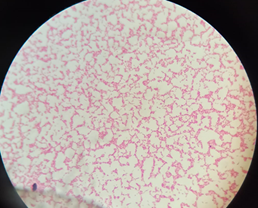
\includegraphics[width=4.3cm]{I2.png} 
	\caption{Imagen de Danna: Tinción de Gram \textit{Escherichia coli} } 
	\label{I1}
	\end{figure} 
	\begin{figure}[!h] 
	\center 
	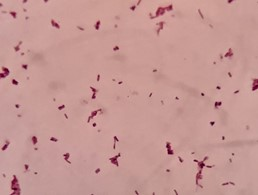
\includegraphics[width=4.3cm]{I6.jpg} 
	\caption{Imagen de Daniela: Tinción de Gram \textit{Escherichia coli} } 
	\label{I1}
	\end{figure} 
	\begin{figure}[!h] 
	\center 
	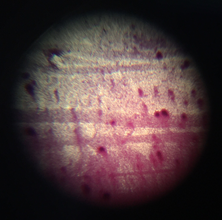
\includegraphics[width=4.3cm]{I10.png} 
	\caption{Imagen de Karen :Tinción de Gram \textit{Escherichia coli} } 
	\label{I1}
	\end{figure} 
	\begin{figure}[!h] 
	\center 
	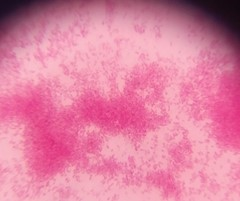
\includegraphics[width=4.3cm]{I14.jpg} 
	\caption{Imagen de William: Tinción de Gram \textit{Escherichia coli} } 
	\label{I1}
	\end{figure} 


\paragraph{\large \textit{\textbf{Staphylococcus aureus}}} Estafilococos Gram positivo
	\begin{figure}[!h] 
	\center 
	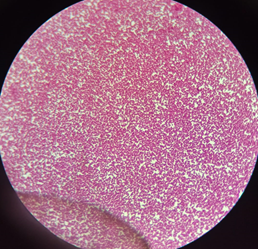
\includegraphics[width=4.4cm]{I3.png} 
	\caption{Imagen de Danna: Tinción de Gram \textit{Staphylococcus aureus} } 
	\label{I1}
	\end{figure} 
	\begin{figure}[!h] 
	\center 
	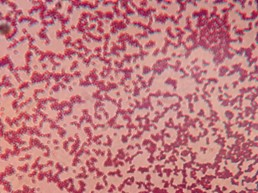
\includegraphics[width=4.2cm]{I7.jpg} 
	\caption{Imagen de Daniela: Tinción de Gram \textit{Staphylococcus aureus} } 
	\label{I1}
	\end{figure} 
	\begin{figure}[!h] 
	\center 
	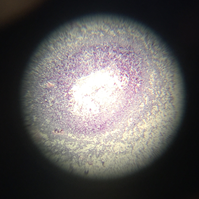
\includegraphics[width=4.2cm]{I11.png} 
	\caption{Imagen de Karen :Tinción de Gram \textit{Staphylococcus aureus} } 
	\label{I1}
	\end{figure} 
	\begin{figure}[!h] 
	\center 
	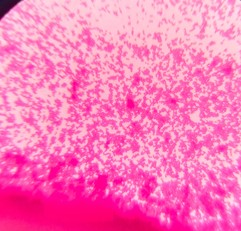
\includegraphics[width=4.2cm]{I15.jpg} 
	\caption{Imagen de William: Tinción de Gram \textit{Staphylococcus aureus} } 
	\label{I1}
	\end{figure} 
\vspace{50mm} 
\paragraph{\large \textit{\textbf{Muestra aleatoria}}}: 
	\begin{figure}[!h] 
	\center 
	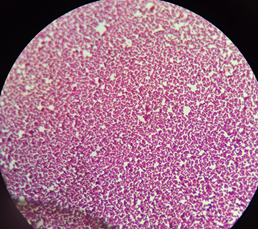
\includegraphics[width=4.9cm]{I4.png} 
	\caption{Imagen de Danna: Tinción de Gram \textit{Muestra aleatoria} } 
	\label{I1}
	\end{figure} 
	\begin{figure}[!h] 
	\center 
	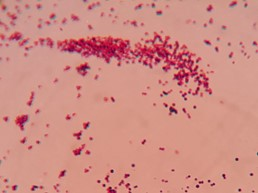
\includegraphics[width=4.2cm]{I8.jpg} 
	\caption{Imagen de Daniela: Tinción de Gram \textit{Muestra aleatoria} } 
	\label{I1}
	\end{figure} 
	\begin{figure}[!h] 
	\center 
	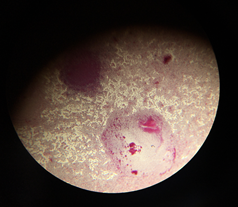
\includegraphics[width=4.2cm]{I12.png} 
	\caption{Imagen de Karen :Tinción de Gram \textit{Muestra aleatoria} } 
	\label{I1}
	\end{figure} 
	\begin{figure}[!h] 
	\center 
	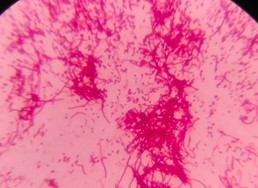
\includegraphics[width=4.2cm]{I16.jpg} 
	\caption{Imagen de William: Tinción de Gram \textit{Muestra aleatoria} } 
	\label{I1}
	\end{figure} 
\vspace{50mm} 
 \subsection{\textbf{Recuento de células en cámara de Neubauer}} 
  
    \begin{figure}[!h] 
	\center 
	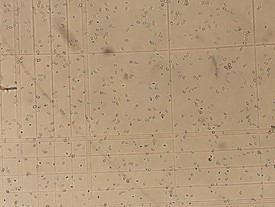
\includegraphics[width=4.5cm]{I17.jpg} 
	\caption{Cámara de recuento de Neubauer bajo el microscopio} 
	\label{I1}
	\end{figure}
	\begin{figure}[!h] 
	\center 
	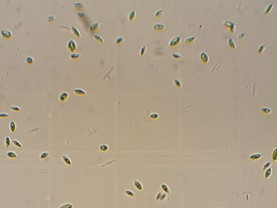
\includegraphics[width=4.5cm]{I18.jpg} 
	\caption{Las microalgas que queremos contar} 
	\label{I1}
	\end{figure}
	
	\vspace{50mm} 
\paragraph{\large \textit{\textbf{Cálculos Zona Roja}}}: 

    \begin{figure}[!h] 
	\center 
	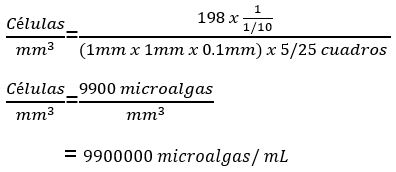
\includegraphics[width=7cm]{I19.jpg} 
	\caption{Cálculos de Danna: Conteo microalgas Zona Roja } 
	\label{I1}
	\end{figure} 
	\begin{figure}[!h] 
	\center 
	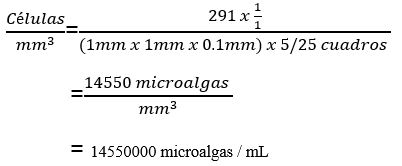
\includegraphics[width=7cm]{I21.jpg} 
	\caption{Cálculos de Daniela: Conteo microalgas Zona Roja} 
	\label{I1}
	\end{figure} 
	\begin{figure}[!h] 
	\center 
	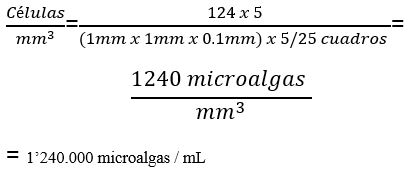
\includegraphics[width=7cm]{I23.jpg} 
	\caption{Cálculos de Karen : Conteo microalgas Zona Roja } 
	\label{I1}
	\end{figure} 
	\begin{figure}[!h] 
	\center 
	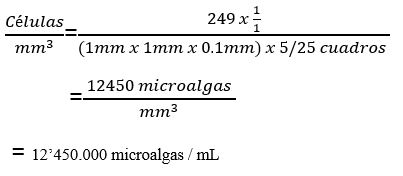
\includegraphics[width=7cm]{I25.jpg} 
	\caption{Cálculos de William: Conteo microalgas Zona Roja } 
	\label{I1}
	\end{figure} 
\paragraph{\large \textit{\textbf{Cálculos Zona Blanca}}}: 
	\begin{figure}[!h] 
	\center 
	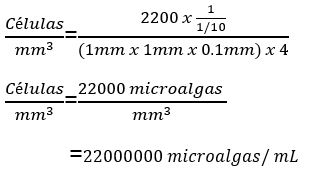
\includegraphics[width=7cm]{I20.jpg} 
	\caption{Cálculos de Danna: Conteo microalgas Zona Blanca } 
	\label{I1}
	\end{figure} 
	\begin{figure}[!h] 
	\center 
	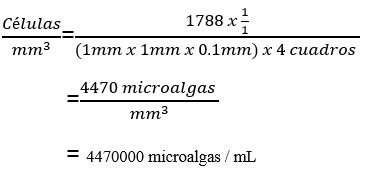
\includegraphics[width=7cm]{I22.jpg} 
	\caption{Cálculos de Daniela: Conteo microalgas Zona Blanca} 
	\label{I1}
	\end{figure} 
	\begin{figure}[!h] 
	\center 
	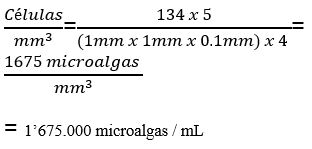
\includegraphics[width=7cm]{I24.jpg} 
	\caption{Cálculos de Karen : Conteo microalgas Zona Blanca } 
	\label{I1}
	\end{figure} 
	\begin{figure}[!h] 
	\center 
	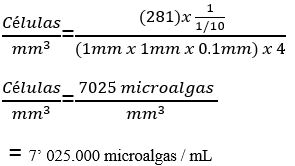
\includegraphics[width=7cm]{I26.jpg} 
	\caption{Cálculos de William: Conteo microalgas Zona Blanca } 
	\label{I1}
	\end{figure}


\section{Análisis y Discusión}
\subsection{\textbf{Tinción de Gram}}
 Dibujar las diferentes observaciones realizadas al microscopio, de los microorganismos coloreados. 
 	\begin{figure}[!h] 
	\center 
	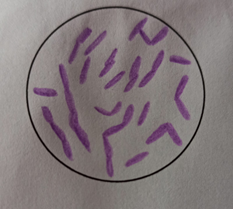
\includegraphics[width=4cm]{I27.png} 
	\caption{Dibujo morfología \textit{Bacillus subtilis} } 
	\label{I1}
	\end{figure} 
	\begin{figure}[!h] 
	\center 
	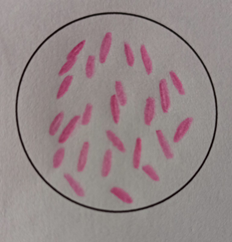
\includegraphics[width=4cm]{I28.png} 
	\caption{Dibujo de morfología \textit{Escherichia coli}} 
	\label{I1}
	\end{figure} 
	\begin{figure}[!h] 
	\center 
	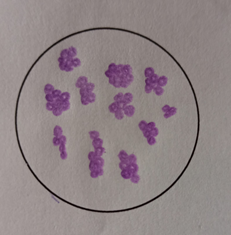
\includegraphics[width=4cm]{I29.png} 
	\caption{Dibujo de morfología \textit{Staphylococcus aureus} } 
	\label{I1}
	\end{figure} 


 Informar correctamente lo observado: 

Bacillus subtilis: Estos se encontraban en mayor cantidad, eran bacilos en cadena, con una coloración morada. 

Escherichia coli: Se observaron con una coloración rosada, no había muchos y además eran tanto diplobacilos como bacilos solos.

Staphylococcus aureus: Se observaron cocos en racimo con una coloración morada, estaban bastante cercanos entre ellos.

Muestra x: Se observaron cocos, algunos diplo, otros en cadena y otros en racimo, tenían una coloración rosada. 

\paragraph{\textbf{Morfología (Ej cocos, bacilos, cocobacilos)}}:

 \begin{itemize}
 \item Bacillus subtilis- Bacilos en cadena
\item Escherichia coli- Diplobacilo
\item Staphylococcus aureus- Cocos
\item Muestra x- Cocos
\end {itemize}
\paragraph{\textbf{Afinidad con la reacción al Gram (Ej. Gram positivos, Gram negativos) }}

 \begin{itemize}
 \item  Bacillus subtilis- Gram positiva
\item Escherichia coli-  Gram negativa
\item Staphylococcus aureus- Gram positiva
\item Muestra x- Gram negativa
\end {itemize}
\paragraph{\textbf{Agrupación}} Generalmente los cocos y los bacilos se agrupan como se describió arriba, por ejemplo en racimo, en cadena o en empalizada. 

R/. Como mencionamos anteriormente, la colonia de Bacillus subtilis encontramos algunos bacilos agrupados en cadena y la E. Coli estaba constituida por diplobacilos. La muestra aleatoria y la muestra de Staphylococcus aureus encontramos bacilos en racimo. 

\paragraph{\textbf{Afinidad con la reacción al Gram (Ej. Gram positivos, Gram negativos)} }


R/. En el caso de los bacillus subtilis, los cuales son bacilos Gram positivos encontramos la presencia de esporas, como se puede ver en la tabla de resultados. 


\section{Cuestionario}
\subsection{\textbf{Tinción de Gram}}
\begin{enumerate}
	\item \textbf{¿Qué significa que las bacterias sean Gram positivas o Gram negativas?¿Porque se tiñen diferente cada uno de esos grupos?}
	
	R/ Las bacterias Gram positivas se tiñen de morado y significa que tienen mayor cantidad de peptidoglicano en su membrana, en cambio las bacterias Gram negativas se tiñen de rosado y tienen menor cantidad de peptidoglicano en su membrana. 
	
	\item \textbf{¿Qué son los microorganismos Gram variables? }
	
	R/ Los microorganismos Gram variables presentan tinción de Gram positivo y de Gram negativo. Algunas bacterias se clasifican como Gram variables, pues simultáneamente presentan tinción de Gram positiva y de Gram negativas, aun bajo condiciones óptimas de cultivo. Sin embargo, en su estructura estas bacterias poseen una pared de Gram positivas, aunque la capa de peptidoglicano es más delgada que la mayoría de bacterias Gram positivas. 
	
	\item \textbf{¿Todas las bacterias se pueden teñir con la coloración de Gram? Explique.}
	
	R/. La coloración de Gram nos permite clasificar a las bacterias en Gram positivas y Gram negativas, sin embargo, hay un grupo de bacterias que debido a la composición de su pared no logran teñirse uniformemente con esta coloración, como lo es el caso de las bacterias ácido alcohol resistentes, las cuales se tiñen por el método Ziehl-Neelsen. 


\item \textbf{Existen bacterias que no se tiñen con la coloración de Gram? En caso positivo explique la razón}

R/. Como se dijo anteriormente, la coloración de Gram nos permite clasificar las bacterias en dos grandes grupos, y aunque hay unas pertenecientes a las BAAR que no se tiñen uniformemente, para obtener un resultado más específico se usa un método especial. 
No existen bacterias que no se logran teñir con esta coloración, sin embargo, sí hay algunas bacterias que poseen estructuras importantes pero que no se logran teñir bien con la coloración de Gram, es por esto que existen otras tinciones como la Leifson-wayson, la Shaeffer-fulton, la tinta china, etc. para poder visualizarlas. 

\end{enumerate}

\subsection{\textbf{Tinciones especiales Ziehl-Neelsen para bacterias ácido alcohol resistentes(B.A.A.R) y Shaeffer-Fulton para esporas bacterianas }}
	
	\begin{enumerate}
	\item \textbf{Defina tinción simple, tinción diferencial y tinción vital, dé algunos ejemplos.}
	
	R/. \textbf{Tinción simple:} Es la tinción que permite únicamente distinguir a las bacterias morfológicamente, utilizando 1 tinte que tiña a las bacterias para poder distinguirlas, o que tiña únicamente el fondo sin teñir a las bacterias. Podremos ver si son cocos, estreptococos, diplobacilos, entre otros. Ejemplos: La mayoría de los colorantes utilizados en las tinciones simples (tinción positiva) son colorantes derivados de las anilinas, sales orgánicas intensamente pigmentadas que proceden del alquitrán. Encontramos el cristal violeta, azul de metileno, safranina, fuchina básica, verde malaquita, rojo Congo, eosina, fuchina ácida, entro muchos otros.

\textbf{Tinción diferencial:}  Es una tinción que permite dividir a las bacterias según sus características celulares y diferenciarlas entre bacterias de distintas especies. Se requiere más de un tinte para estos tipos de tinción. Ejemplos: Tinción de Gram, Tinción de Ziehl-Neelsen.

\textbf{Tinción vital:} Las tinciones vitales son tinciones hematológicas que se realizan sobre células vivas, manteniéndose en dicho estado. La técnica se basa en la introducción de un colorante en la circulación de un organismo vivo. Los organismos microscópicos, como los protozoos, pueden ser inmersos totalmente en una solución colorante. Ejemplos:  El verde Jano, las sales de tetrazolio o el azul de metileno son ejemplos de colorantes vitales. (Rodríguez, 2021)

	
	\item \textbf{Defina tinción negativa y tinción positiva. }
	
	R/. \textbf{Tinción negativa:} Es una tinción que permite visualizar la cápsula de los microorganismos. Se basa en teñir el fondo del frotis en un color oscuro. En este escenario las estructuras capsuladas resaltan en color claro o incoloro. Esto ocurre porque la tinta china y la nigrosina son sustancias incapaces de penetrar el polisacárido que conforma la cápsula de los microorganismos vivos. Ahora bien, si los microorganismos están muertos, la tintura puede penetrar dentro de los mismos, de tal manera que esta tinción también es útil para evaluar la viabilidad de los microorganismos (Gil, 2017). El principio de esta técnica es no teñir al microorganismo, pero en vez teñir el fondo.
	
\textbf{Tinción positiva:} A diferencia de la tinción negativa, esta utiliza tintes para teñir el microorganismo en contra de un fondo brillante. El tipo de tinte usado en esta técnica es un ion cargado positivamente. La pared celular cargada negativamente de muchos microorganismos atrae el cromóforo cargado positivamente que hace que la muestra absorba la tinta, dándole al microorganismo este color.
Una tinción positiva es aquélla en la que se observan bacilos ácido-alcohol resistentes, los cuales son de color rojo fucsia. 

\item \textbf{Averiguar el fundamento de la Tinción de ZN }

R/. Se basa en identificación de la pared celular de los microorganismos AAR, la pared está formada por unos ácidos grasos llamados ácidos micólicos, además de tener cadenas muy largas, esto les permite retener el colorante. En la tinción ZN se utiliza el fenólico carbol fucsina, este tiene la capacidad de interactuar con los ácidos grasos de la pared celular, cuando se le añade calor esta se derrite y las moléculas se mueven más rápido hacia el interior de la pared celular.

\item \textbf{Definir baciloscopia, sus indicaciones de realización y la forma correcta de reporte. }

R/. La baciloscopia es una prueba de tipo diagnóstico que se realiza para detectar la presencia de bacilos en una muestra biológica mediante visualización en microscopio. Este análisis permite encontrar actividad de bacilos ácido alcohol resistentes como el que produce la enfermedad de la tuberculosis, llamado Mycobacterium tuberculosis. Para lograr su detección se utiliza una técnica especial de tinción conocida como Ziehl-Neelsen.

Para la realización de este examen debes tomar aire profundamente, llenando tus pulmones de aire tanto como sea posible, y retenlo un momento. Tose fuertemente dentro del frasco, con el fin de que salga la flema de tu garganta. Evita derramar la muestra por fuera del recipiente. Es ideal que la muestra tenga consistencia de moco y con poca saliva.

	\item \textbf{¿Qué son los gránulos metacromáticos?¿En qué bacterias se encuentran?}
	
	R/. Los gránulos metacromáticos son gránulos de reserva, normalmente fosfatos inorgánicos utilizados en la síntesis, que suelen ser de gran tamaño. Se encuentran en bacterias de los géneros Corynebacterium y Mycobacterium.

	\end{enumerate}
	

\subsection{\textbf{Metodos de siembra y caracterización morfológica de hongos (micromicetos filamentosos) }}
	
	\begin{enumerate}
	\item \textbf{¿Cómo se clasifica la tinción de azul de lactofenol?}
	
	R/. Está clasificado como peligroso, con toxicidad aguda de categoría 4, ya sea oral, inhalación o cutáneo, tiene corrosión cutánea categoría 1B, mutagenicidad en células germinales categoría 2 y toxicidad específica en determinados órganos categoría 3.
	

	\item \textbf{¿Cuál es el fundamento de la tinción de azul de lactofenol para observación de hongos al microscopio?}
	
	R/ Se realiza una coloración simple de las estructuras fúngicas, este actúa como clarificante de la muestra, por su acción de ácido láctico con fenol. El fenol se comporta como como un mordiente y evita la lisis del microorganismo al inhibir las enzimas hidrolíticas presentes; mientras tanto el ácido láctico preserva la morfología de las estructuras del hongo. Además, este tiñe el citoplasma y la quitina (azul claro) presente en la célula fúngica.

	
	\item \textbf{¿Cuál es el fundamento del agar Saboureaud + cloranfenicol?}
	
	R/. Medio de cultivo recomendado para el aislamiento y desarrollo de hongos, particularmente los asociados con infecciones cutáneas (piel, pelo). En el medio de cultivo, la peptona, la tripteína y la glucosa son los nutrientes para el desarrollo de microorganismos. El alto contenido de glucosa, la presencia de cloranfenicol y el pH ácido, inhiben el desarrollo bacteriano y favorecen el crecimiento de hongos y levaduras. El agar es el agente solidificante. Puede ser suplementado con otros agentes selectivos de crecimiento.

	
	
	\item \textbf{Según el fundamento… ¿Por qué algunos micelios se denominan hialinos y otros dematiáceos?}
	
	R/. Algunos micelios se denominan hialinos por ser incoloros, es decir que necesitan de una tinción, en este caso azul de lactofenol, para poder ser visibles a través del microscopio. Por otro lado, los dematiáceos presentan un color gris oscuro, marrón o negro, y no son transparentes como los hialinos, por lo cual no es estrictamente necesario utilizar una tinción con este tipo de hongos. 
	
	\item \textbf{En una coloración de Gram, ¿Cómo diferencio una levadura de una bacteria?}
	
	R/. Existe una gran diversidad de especies de levaduras y bacterias. Por este motivo, las creencias como que las colonias de levaduras son alargadas y las de bacterias son redondas, o incluso que las bacterias crecen de color rojo en un medio con TTC (Cloruro de Trifenil Tetrazolio) y las levaduras no; son simplificaciones que dan lugar a errores. Todas las levaduras son Gram positivas, pero la mejor forma de diferenciarlas es utilizar un medio de cultivo diferencial con antibacterianos de amplio espectro (que ataca zonas de ADN comunes para muchas especies de bacterias ) como el Cloranfenicol , al que para estar más seguros podemos añadir otro agente antibacteriano de amplio espectro que ataque la pared bacteriana, como la Oxitetraciclina (Lab. MicroKit, n.d.).

	
\end{enumerate}

\section{Conclusión}
	
	\begin{enumerate}[label=(\roman*)]
	
    \item Se logró determinar la morfología y la afinidad a la tinción Gram de diferentes microorganismos después de observar en el microscopio.
    \item  Pudimos determinar que microorganismos eran Gram positivos y Gram negativos. 
    
    \item  Se realizó un buen conteo de microalgas utilizando la cámara de Neubauer, y se realizaron los respectivos cálculos teniendo en cuenta el factor de dilución y los cuadrantes y cuadros contados para cada zona. 
    \item Profundizamos en algunos temas vistos en clase como las tinciones especiales y la caracterización morfológica para hongos, esto nos ayudó a diferenciar distintos microorganismos dentro del informe y entender mejor cada uno de los procedimientos para su correspondiente identificación

   
	\end{enumerate}

\appendices


\ifCLASSOPTIONcaptionsoff
  \newpage
\fi


\begin{thebibliography}{1}


 \bibitem{IEEEhowto:Monteria}
  Rodríguez, F., 2017. Tinciones hematológicas - Blog de Laboratorio Clínico y Biomédico. [online] Blog de Laboratorio Clínico y Biomédico. Available at: $https://www.franrzmn.com/tinciones-hematologicas/$ [Accessed 11 October 2021].
 

 \bibitem{IEEEhowto:Monteria}
 Marielsa Gil. (18 de enero de 2019). Tinción negativa: fundamento, técnica, ventajas y desventajas. Lifeder. Recuperado de https://www.lifeder.com/tincion-negativa/ Bacterias gram. (n.d.). Retrieved September 20, 2021, from https://es.slideshare.net/renxsparza/bacterias-gram-38151652 
 
 \bibitem{IEEEhowto:Monteria}
 Gil, M. (2019, 30 octubre). Azul de lactofenol: características, composición, preparación, usos. Lifeder. https://www.lifeder.com/azul-de-lactofenol/

 
 \bibitem{IEEEhowto:Monteria}
 Lopez, L., Hernandez, M., Colin, C., Ortega, S., Franco, R. (2014). Las tinciones básicas en el laboratorio de microbiología. Medigraphic, 3(1), 10–18. $https://www.medigraphic.com/pdfs/invdis/ir-2014/ir141b.pdf$
 
 
 \bibitem{IEEEhowto:Monteria}
 Pontificia universidad javeriana. (2015, 10 noviembre). AZUL DE LACTOFENOL [Tarjeta de emergencia]. 29cd622e-8677-40b2-b25d-6f900456282e. 
 https://www.javeriana.edu.co/documents/4486808/5015296/AZUL+DE+
 LACTOFENOL+T.E..pdf/29cd622e-8677-40b2-b25d-6f900456282e?version=1.0

 
 \bibitem{IEEEhowto:Monteria}
 Ochoa, A. (2014, 26 enero). Célula Bacteriana [Diapositivas]. Slideshare. https://es.slideshare.net/gabitaochoa/celula-bacteria
 
 \bibitem{IEEEhowto:Monteria}
 Briceño, K. (2021, 19 febrero). Tinción de Ziehl-Neelsen. Lifeder. https://www.lifeder.com/tincion-ziehl-neelsen/

 \bibitem{IEEEhowto:Monteria}
 
 Baciloscopia | Christus Muguerza. (n.d.). Retrieved October 10, 2021, from https://www.christusmuguerza.com.mx/laboratorio/baciloscopia

 \bibitem{IEEEhowto:Monteria}
 
 Lab. MicroKit, n.d. [online] Microkit.es. Available at: <https://www.microkit.es/pdf/pre-identificacion.pdf> [Accessed 11 October 2021] 

 
 
 
\end{thebibliography}



\end{document}
